\documentclass[10pt,aspectratio=169]{beamer}
% \documentclass[10pt,aspectratio=169,handout]{beamer}

% silence some Metropolis warnings
\usepackage{silence}
\WarningFilter{beamerthememetropolis}{You need to compile with XeLaTeX or LuaLaTeX}
\WarningFilter{latexfont}{Font shape}
\WarningFilter{latexfont}{Some font}

% define custom colors
\definecolor{dark gray}{HTML}{444444}
\definecolor{light gray}{HTML}{777777}
\definecolor{dark red}{HTML}{BB0000}
\definecolor{dark green}{HTML}{00BB00}

% configure metropolis
\usetheme[numbering=fraction]{metropolis}
\setbeamercolor{background canvas}{bg=white}
\setbeamercolor{frametitle}{bg=dark gray}
\setbeamercolor{alerted text}{fg=dark red}
\setbeamercolor{item projected}{bg=dark red}
\setbeamercolor{local structure}{fg=dark red}
\setbeamersize{text margin left=0.5cm,text margin right=0.5cm}
\setbeamercovered{transparent=10}

% use thicker lines
\makeatletter
\setlength{\metropolis@titleseparator@linewidth}{1pt}
\setlength{\metropolis@progressonsectionpage@linewidth}{1pt}
\makeatother

% custom bullet points
\setbeamertemplate{itemize item}{\color{dark red}$\blacktriangleright$}
\setbeamertemplate{itemize subitem}{\color{dark red}$\blacktriangleright$}
\setbeamertemplate{itemize subsubitem}{\color{dark red}$\blacktriangleright$}
\newcommand{\custombullet}{{\color{dark red}$\blacktriangleright$}\hspace{0.5em}}

% use classic font for math
\usefonttheme[onlymath]{serif}

% imports
\usepackage[english]{babel}
\usepackage[utf8]{inputenc}
\usepackage{amsthm}
\usepackage{amssymb}
\usepackage{amsmath}
\usepackage{amsfonts}
\usepackage{mathtools}
\usepackage{mathabx}
\usepackage{stmaryrd}
\usepackage{graphicx}
\usepackage{hyperref}
\usepackage{xfrac}
\usepackage{appendixnumberbeamer}

% check and x marks
\usepackage{pifont}
\newcommand{\cmark}{{\color{dark green}\ding{51}}\hspace{0.3em}}
\newcommand{\xmark}{{\color{dark red}\ding{55}}\hspace{0.5em}}

% diagrams
\usepackage{tikz}
\usetikzlibrary{decorations.pathreplacing}

% references
\usepackage[natbibapa]{apacite}
\bibliographystyle{apacite}
\renewcommand{\bibsection}{}

% use ampersands instead of "and" for text citations
\AtBeginDocument{\renewcommand{\BBAB}{\&}}

% possessive cites
\makeatletter
\patchcmd{\NAT@test}{\else \NAT@nm}{\else \NAT@nmfmt{\NAT@nm}}{}{}
\DeclareRobustCommand\citepos
  {\begingroup
   \let\NAT@nmfmt\NAT@posfmt
   \NAT@swafalse\let\NAT@ctype\z@\NAT@partrue
   \@ifstar{\NAT@fulltrue\NAT@citetp}{\NAT@fullfalse\NAT@citetp}}
\let\NAT@orig@nmfmt\NAT@nmfmt
\def\NAT@posfmt#1{\NAT@orig@nmfmt{#1's}}
\makeatother

% spaced-out lists
\newenvironment{wideitemize}{\itemize\addtolength{\itemsep}{10pt}}{\enditemize}
\newenvironment{wideenumerate}{\enumerate\addtolength{\itemsep}{10pt}}{\endenumerate}

% replace footnotes with buttons
\usepackage[absolute,overlay]{textpos}
\newcounter{beamerpausessave}
\newcommand{\always}[1]{
    \setcounter{beamerpausessave}{\value{beamerpauses}}
    \setcounter{beamerpauses}{0}
    \pause
    #1 
    \setcounter{beamerpauses}{\value{beamerpausessave}}
    \addtocounter{beamerpauses}{-1}
    \pause
}
\newcommand{\buttons}[1]{\always{
    \begin{textblock*}{\paperwidth}(0.015\textwidth, 1.022\textheight)
        \scriptsize
        #1
    \end{textblock*}
}}
\newcommand{\appendixbuttons}[1]{\always{
    \begin{textblock*}{\paperwidth}(0.015\textwidth, 1.043\textheight)
        \scriptsize
        #1
    \end{textblock*}
}}
\newcommand{\goto}[2]{\hyperlink{#1}{{\color{dark red}$\smalltriangleright$} #2}\hspace{0.5em}}
\newcommand{\goback}[2]{\hyperlink{#1}{{\color{dark red}$\smalltriangleleft$} #2}\hspace{0.5em}}

% custom appendix
\renewcommand{\appendixname}{\texorpdfstring{\translate{Appendix}}{Appendix}}

% change color of cites and URLs
\let\oldcite\cite
\let\oldcitet\citet
\let\oldcitep\citep
\let\oldcitepos\citepos
\let\oldcitetalias\citetalias
\let\oldcitepalias\citepalias
\let\oldurl\url
\def\cite#1#{\citeaux{#1}}
\def\citet#1#{\citetaux{#1}}
\def\citep#1#{\citepaux{#1}}
\def\citepos#1#{\citeposaux{#1}}
\def\citetalias#1#{\citetaliasaux{#1}}
\def\citepalias#1#{\citepaliasaux{#1}}
\def\url#1#{\urlaux{#1}}
\newcommand*\citeaux[2]{{\color{light gray}\oldcite#1{#2}}}
\newcommand*\citetaux[2]{{\color{light gray}\oldcitet#1{#2}}}
\newcommand*\citepaux[2]{{\color{light gray}\oldcitep#1{#2}}}
\newcommand*\urlaux[2]{{\color{light gray}\oldurl#1{#2}}}
\newcommand*\citeposaux[2]{{\color{light gray}\oldcitepos#1{#2}}}
\newcommand*\citetaliasaux[2]{{\color{light gray}\oldcitetalias#1{#2}}}
\newcommand*\citepaliasaux[2]{{\color{light gray}\oldcitepalias#1{#2}}}

% custom math commands
\DeclareMathOperator*{\argmax}{argmax}
\DeclareMathOperator*{\argmin}{argmin}
\renewcommand{\Pr}{\mathbb{P}}
\newcommand{\E}{\mathbb{E}}
\newcommand{\Var}{\mathbb{V}}
\newcommand{\Cov}{\mathbb{C}}
\newcommand{\overbar}[1]{\mkern 1.5mu\overline{\mkern-1.5mu#1\mkern-1.5mu}\mkern 1.5mu}

% tables
\usepackage{booktabs}
\usepackage{colortbl}
\usepackage{multirow}
\usepackage{makecell}
\arrayrulecolor{dark red}

% custom date
\usepackage{datetime}
\newdateformat{monthyeardate}{\monthname[\THEMONTH] \THEYEAR}

% fix pauses with graphics
\usepackage{fixpauseincludegraphics}


\title []{Vertical Control}
\author{C.Conlon }
\institute{Grad IO }
\date{Fall 2022}
\setbeamerfont{equation}{size=\tiny}
\begin{document}

\begin{frame}
\titlepage
\end{frame}




%%%%%%%%%%%%%%%%%%%%%%%%%%%%%%%%%%%%%%%%%%%%%%%%%%
%%%%%%%%%%%%%%%%%%%%%%%%%%%%%%%%%%%%%%%%%%%%%%%%%%%
\section{Overview}


\begin{frame}{Readings}
\begin{itemize}
\item If you haven't worked through double marginalization, read Chapter 4 of Tirole
\item You should read the chapter from Whinston's antitrust lectures.
\item Exclusionary Contracts: Conlon Mortimer (JPE 2021)
\item Bargaining Models in Healthcare: Ho and Lee (AER 2019), Gowrisankaran, Nevo Town (AER 2015).
\item Bargaining in TV: Crawford, Lee, Whinston, Yurukoglou (ECMA 2018), Crawford Yurukoglou (AER 2012)
\item Do upstream or downstream firms set prices (Villas Boas (2007), Bonnet and Dubois (2010)).
\end{itemize}
\end{frame}

\frame[plain]{ 
\frametitle{Vertical Control}

Manufacturers rarely supply final consumers directly (as we have modeled them so far).  
Instead, most industries are vertically separated.\\  
\vspace{0.2in} 
We often refer to firms in these markets as upstream and downstream firms.  In these settings, 
downstream firms are the customers of the upstream firms, and many of the standard issues 
still apply.  For example:\\
\begin{enumerate}
\item choice of price is endogenous\\
\item price discrimination (both the upstream and downstream firms)\\
\item mergers\\
\item entry, etc.\\ 
\end{enumerate}
}

\frame[plain]{
\frametitle{Vertical Control}

However, things can also get more complicated in vertically separated environments.  In particular, downstream firms 
do not usually consume the good, but typically make further decisions regarding the product.\\ 
\vspace{0.2in}
Examples of activities of downstream firms:\\
\begin{enumerate}
\item determination of final price\\
\item promotional effort\\
\item placement of product on store shelves\\
\item promotion and placement of competing products\\
\item technological inputs\\
\end{enumerate}
}

\frame[plain]{
\frametitle{Vertical Control}
Why don't manufacturers simply engage in direct marketing to consumers?\\
\vspace{0.2in}
Some reasons:\\
\begin{enumerate}
\item increasing returns to distribution due to shopping needs or travel costs for consumers\\
\item choice of variety\\
\item demand for service \\
\item integration of complementary products\\
\item different geographical markets, etc. 
\end{enumerate}
}

\frame[plain]{
\frametitle{Vertical Control}
Unlike the consumption activities of final consumers, the activities of the downstream firms may affect the profits of the upstream firm.\\
\vspace{0.2in}
This is why upstream firms care about the activities of the downstream firms, and why we study vertical control/restraints between firms in these settings.\\
\vspace{0.2in}
We focus on the incentives for vertical control when the market for the intermediate good is imperfectly competitive.\\
}
\frame[plain]{
\frametitle{Vertical Control}
A common benchmark for what firms can achieve through vertical control is the ``vertically integrated profit.''  This is the maximum industry or aggregate (manufacturer plus retailer) profit.  \\
\vspace{0.2in}
If firms use vertical restraints efficiently, they should achieve the vertically integrated profit.\\
}

\frame[plain]{
\frametitle{Vertical Control}

There are several types of vertical restraints used by firms in vertically-separated markets:\\
\begin{enumerate}
\item {\it Exclusive Territories}: a dealer/ distributor/ retailer is assigned a (usually geographic) territory by the manufacturer/ upstream firm and given monopoly rights to sell in that area. [e.g Car Dealerships, Franchises, Beverage Distributors]\\
\vspace{0.2in}
\item {\it Exclusive Dealing}:  a dealer/ distributor/ retailer is not allowed to carry the brands of a competing upstream firm.[See Asker 2005 or Sass 2004,2005] on beer distribution.
\vspace{0.2in}
\item {\it Full-line forcing}:  a dealer is committed to sell all the varieties of the manufacturer's products rather than a limited selection.  (i.e., the upstream firm ties all its products to sell to the downstream firm). See [Ho, Ho, Mortimer AER 2012] on video rentals.\\
\end{enumerate}
}

\frame[plain]{
\frametitle{Vertical Control}
\begin{enumerate}
\setcounter{enumi}{3}
\item {\it Resale Price Maintenance}:  a dealer commits to a retail price or a range of retail prices for the product.  This can 
take the form of either minimum resale price maintenance or maximum resale price maintenance.  Equivalently, firms can engage in quantity forcing or quantity rationing. [Apple (appears to have) minimum RPM for it's products]
\vspace{0.2in}
\item {\it Contractual arrangements}:  upstream and downstream firms write contracts to provide greater flexibility in the transfer 
of the product.  Profit sharing and revenue sharing [Mortimer ReStud 2008] are the most common, which we'll see soon.  Also, franchising arrangements.\\
\end{enumerate}
}

\frame[plain]{
\frametitle{Legal Issues}
%Legal Issues
\vspace{0.1in}
\begin{itemize}
\item There are many ambiguities in the legal treatment of vertical contracts.\\
\vspace{0.1in}
\item Until 1970s, RPM and E. Territories were \underline{per se}
illegal under Sherman Act.\\
\vspace{0.1in}
\item But many states passed fair trade laws that were interpreted to
cover some of these cases.\\
\vspace{0.1in}
\item Furthermore, the Khan case in 1997 switched Maximum RPM to a ``rule of reason'' status, as did the Leegin Leather Products case in 2007 for Minimum RPM.\\
\end{itemize}
}

\frame[plain]{
\frametitle{Legal Issues}

Thus, although price fixing remains \underline{per se} illegal,
it's not always applied in vertical settings because it conflicts with
free-trade notions between mfgs and their distributors.\\
\vspace{0.2in}
Non-price issues have been generally accepted to be ok by the
courts.  Decisions turn on arguments about efficiency vs. anti-competitive effects.\\
\begin{itemize}
\item Exclusive territories 
\item Refusal to deal 
\item Foreclosure, etc.
\end{itemize}
}

\frame[plain]{
\frametitle{Further Reading}
Understanding the legal framework is important for working with vertical restraints:
\begin{itemize}
\item John Kwoka and Larry White (NYU Stern) have compiled an edited volume of summarized IO economist testimony and reports from various cases in \textit{The Antitrust Revolution} across soon to be 7 volumes.
\item Whinston has written some nice lectures on Antitrust, and Chapter 4 focuses specifically on vertical issues.
\item There is not much on legal details, but Tirole's \textit{Theory of Industrial Organization} covers many theoretical models on vertical contracting.
\end{itemize}

}


\frame[plain]{
\frametitle{Vertical Control}
The typical outline of vertical control is as follows:\\
\begin{enumerate}
\item Double Marginalization/Successive Monopoly Problem.

\item Externalities between downstream and upstream firms (Maximum Resale Price Maintenance, Quantity Forcing, Contractual Arrangements, or Full-line Forcing)\\

\item Downstream Moral Hazard, or Externalities from Intrabrand competition (Exclusive Territories, Minimum RPM, or Quantity Rationing)\\

\item Interbrand competition (Exclusive Dealing or possibly Full-line Forcing)\\
\end{enumerate}
}

\section{Basic Framework}

\frame[plain]{
\small
\frametitle{Double Marginalization}
\begin{itemize}
\item $U$ sells product to $D$ who sells product to final consumers.
\item Homogeneous product with final demand given by $D(p_d)$.
\item $U$ charges $p_w$ to $D$.
\item $D$ chooses how much to buy from $U$
\begin{eqnarray*}
\max_{p_d} \pi_d &\equiv& \max_{p_d} (p_d-p_w) D(p_d) \\
\mbox{ FOC: }&&  (p_d - p_w) D'(p_d) + D(p_d) = 0
\end{eqnarray*}
\item The solution is denoted by $p_d^*(p_w)$
\item The upstream firm $(U)$ now solves:
\begin{eqnarray*}
\max_{p_w} \pi_w &\equiv& \max_{p_w} (p_w-c ) D(p_d^*(p_w)) 
\end{eqnarray*}
\item We have that $p_w  > c$ and $p_d > p_w$ which we call \alert{double marginalization}.
\end{itemize}
}



\frame[plain]{
\frametitle{Externalities}



\begin{picture}(5,35)(-40,-5)
\setlength{\unitlength}{1mm}

\linethickness{1pt}
% this one is horizontal
\put(-5,-35){\line(1,0){85}}
% this one is vertical
\put(-5,-35){\line(0,1){70}}
%labels
\put(-10,35){\makebox(0,0)[l]{$P$}}
\put(85,-35){\makebox(0,0)[r]{$Q$}}

%this one is demand
\put(-5,25){\line(4,-3){85}}
\put(80,-41){\makebox(0,0)[r]{$D_r$}}
%this one is marginal revenue
\put(-5,25){\line(2,-3){42.5}}
\put(45,-41){\makebox(0,0)[r]{$MR_r=D_w$}}
%this one is marginal revenue #2
\put(-5,25){\line(1,-3){21.25}}
\put(20,-41){\makebox(0,0)[r]{$MR_w$}}
% this one is marginal cost
\put(-5,-25){\line(2,0){70}}
\put(72,-25){\makebox(0,0)[r]{$MC$}}
% this one is wholesale price
%\put(-5,0){\line(2,0){33.5}}
%%%%%
\qbezier[13](-5,0)(3.5,0)(12,0)
%\put(70,0){\makebox(0,0)[r]{\tiny{$wholesale \, price$}}}
\put(-11,0){\makebox(0,0)[l]{$P_w$}}


%this one is VI choice of q
%%\qbezier[25](28,5,-35)(28.5,-17.5)(28.5,0)
%this is 2nd monopoly choice of q
\qbezier[25](12,-25)(12,-8.75)(12,12.5)
%this is retail price
\qbezier[13](-5,12.5)(3.5,12.5)(12,12.5)
\put(-10,12.5){\makebox(0,0)[l]{$P_r$}}

\linethickness{1pt}
% this one is horizontal
%%\put(-5,-35){\line(2,0){85}}
% this one is vertical
%%\put(-5,-35){\line(0,2){70}}
%labels
%%\put(-10,30){\makebox(0,0)[l]{\tiny{$P$}}}
%%\put(85,-35){\makebox(0,0)[r]{\tiny{$Q$}}}

%this one is demand
%%\put(-5,25){\line(4,-3){85}}
%%\put(80,-40){\makebox(0,0)[r]{\tiny{$D_r$}}}
%this one is marginal revenue
%%\put(-5,25){\line(2,-3){42.5}}
%%\put(45,-40){\makebox(0,0)[r]{\tiny{$MR_r=D_w$}}}
%this one is marginal revenue #2
%%\put(-5,25){\line(1,-3){22.25}}
%%\put(20,-40){\makebox(0,0)[r]{\tiny{$MR_w$}}}
% this one is marginal cost
%%\put(-5,-25){\line(2,0){140}}
%%\put(70,-25){\makebox(0,0)[r]{\tiny{$MC$}}}
% this one is wholesale price
%\put(-5,0){\line(2,0){33.5}}
\qbezier[25](-5,0)(12,0)(28.5,0)
%\put(70,0){\makebox(0,0)[r]{\tiny{$wholesale \, price$}}}
%%\put(-10,0){\makebox(0,0)[l]{\tiny{$P_w$}}}


%this one is VI choice of q
\qbezier[25](28.5,-35)(28.5,-17.5)(28.5,0)
%this is 2nd monopoly choice of q
%%\qbezier[50](12,-25)(12,-8.75)(12,12.5)
%this is retail price
%%\qbezier[25](-5,12.5)(3.5,12.5)(12,12.5)
%%\put(-10,12.5){\makebox(0,0)[l]{\tiny{$P_r$}}}

\end{picture}
}

\frame[plain]{
\small
\frametitle{Double Marginalization}
\begin{itemize}
\item Double Marginalization arises from the externality as $p_w$ raises his price this raises the effective marginal cost to $U$ and the monopoly price she charges is too large.
\item Think about a vertically integrated firm.
\begin{eqnarray*}
\max_{p_m} \pi_d &\equiv& \max_{p_m} (p_m-c) D(p_m) \\
\mbox{ FOC: }&&  (p_m - c) D'(p_m) + D(p_m) = 0
\end{eqnarray*}
\item Since $p_w > c$ then we have that $\pi_D + \pi_U < \pi_{VI}$ and $p_D^*(p_w) > p^*(c)$
\end{itemize}
}


\frame[plain]{
\small
\frametitle{Double Marginalization}
Most solutions involve contracting around the externality:
\begin{itemize}
\item Consider a \alert{two-part tariff} where $p_w = c$ but that $\widetilde{\pi_D} =\pi_D -T$ and  $\widetilde{\pi_U} =\pi_U +T$. We call $T$ the \alert{franchise fee}. This is sometimes known as the \alert{sell out contract} because the wholesaler sets $p_w=c$. 
\item Now we have that $\widetilde{\pi_D} = \pi_{VI} - T$ and $\widetilde{\pi_U} = 0 + T$.
\item There are other (sometimes legal, sometimes not solutions): \alert{RPM} to set $p_d^* = p^m.$
\item \alert{Quantity Forcing}. Upstream firm makes a TILO offer of monopoly quantity to $D$.
\item We can also allow \alert{revenue or profit sharing } where $U$ ``owns'' a fraction $\lambda$ of the upstream firm.
\begin{itemize}
\item These contracts are common in franchises. (ie: Subway corporate keeps 20\% of your revenue).
\end{itemize}
\end{itemize}
}


\frame[plain]{
\small
\frametitle{Challenges for  Empirical Work}
\begin{itemize}
\item Good empirical work on these topics is generally limited by the availability of data
\item It is not too difficult to gather data on retail $(P,Q)$.
\item Wholesale prices are harder to observe.
\item Most nonlinear contracts between upstream and downstream firms are closely guarded trade secrets.
\item If you can get your hands on contracts, you can write papers!
\end{itemize}
}

\begin{frame}{Villas Boas (ReStud 2007)}
Retailer and Wholesaler FOC given by:
\begin{align*}
\mathbf{p^r} &= \underbrace{\mathbf{p^w} +\mathbf{c^r}}_{\mathbf{mc^r}} -(\mathcal{H}_r \odot \Delta_{r}(\mathbf{p^r}))^{-1} \mathbf{s}(\mathbf{p^r})\\
\mathbf{p^w}  &= \mathbf{mc^w} + \left(\mathcal{H}_{w} \odot \left( \frac{\partial \mathbf{p^r}}{\partial \mathbf{p^w}} \cdot  \Delta_r(\mathbf{p^r} ) \right) \right)^{-1} \mathbf{s}(\mathbf{p^r})
\end{align*}
\begin{itemize}
  \item $\Delta_r$ is matrix of (retail) demand derivatives $\frac{\partial\, \mathbf{s}}{\partial\, \mathbf{p}}$.
\item $\mathcal{H}_r,\mathcal{H}_w$  ownership matrix $(j,k)=1$ if both products sold by same retailer/wholesaler.
\item $\frac{\partial\, \mathbf{p^r}}{\partial\, \mathbf{p^w}}$ is the \alert{pass-through matrix} (NEW!)
\end{itemize}
Challenge: We want $\mathbf{p^r}(\mathbf{p^w})$ and $\mathbf{mc^w}$ but we only have implicit solution for retailer FOC.
\end{frame}

\begin{frame}{How do we get pass-through?}
The \alert{pass-through matrix} $\frac{\partial \mathbf{p^r}}{\partial \mathbf{p^w}}$ can be obtained in one of two ways:
\begin{enumerate}
\item Numerically: perturbing the retailer's marginal costs for each possible choice of $k$ and solving
\begin{align*}
\mathbf{p^r} &=\mathbf{mc^r} + e_k -(\mathcal{H}_r \odot \Delta_{r}(\mathbf{p^r}))^{-1} \mathbf{s}(\mathbf{p^r})\\
\end{align*}
(Use Morrow Skerlos (2011) formulation and solve for every $(j,k)$ pair).
\item Analytic: Use the retailer's FOC and apply the implicit function theorem.
\begin{align}
\tag{retailer FOC}
 f(\mathbf{p^r},\mathbf{mc^r}) &\equiv \mathbf{p^r}  - \mathbf{mc^r}-  \left(\mathcal{H}_{r} \odot \Delta(\mathbf{p^r}) \right)^{-1} \mathbf{s}(\mathbf{p^r})=0 
\end{align}
See Jaffe Weyl (AEJM 2013) or Miller Weinberg (2017 Appendix E) or Conlon Rao (2022).\\
\alert{This is what PyBLP does}.
  \end{enumerate}

\end{frame}

\begin{frame}{Multivariate IFT: Easy Part}
The multivariate IFT says that for some system of $J$ nonlinear equations 
\begin{align*}
f(\mathbf{p^r},\mathbf{p^w}) \equiv [F_1(\mathbf{p^r},\mathbf{p^w}), \ldots, F_J(\mathbf{p^r},\mathbf{p^w})]=[0,\ldots,0]
\end{align*}
with $J$ endogenous variables $\mathbf{p^r}$ and $J$ exogenous parameters $\mathbf{p^w}$.
\begin{align}
\label{eq:ptr_matrix}
\tag{PTR}
\frac{\partial \mathbf{p^r}}{\partial \mathbf{p^w}}
=-\left(\begin{array}{ccc}
\frac{\partial F_{1}}{\partial p_{1}^r} & \ldots & \frac{\partial F_{1}}{\partial p_{J}^r} \\
\ldots & \ldots & \ldots \\
\frac{\partial F_{J}}{\partial p_{1}^r} & \ldots & \frac{\partial F_{J}}{\partial p_{J}^r}
\end{array}\right)^{-1} \cdot \underbrace{\left(\begin{array}{l}
\frac{\partial F_{1}}{\partial p_{k}^w} \\
\ldots \\
\frac{\partial F_{J}}{\partial p_{k}^w}
\end{array}\right)}_{= -\mathbb{I}_J}
\end{align}
Because the system of equations is additive in $\mathbf{mc^r} = \mathbf{c^r} + \mathbf{p^w}$ this simplifies dramatically.
\end{frame}


\begin{frame}{Multivariate IFT: Hard Part}
Use the substitution $\Omega(\mathbf{p^r}) \equiv \mathcal{H}_r \odot \Delta_{r}(\mathbf{p^r})$, and differentiate the wholesalers' system of FOC's with respect to $p_l$, to get the $J \times J$ matrix with columns $l$ given by:
\begin{align}
\frac{\partial f(\mathbf{p^r},\mathbf{p^w})}{\partial p_l^r} \equiv e_l - \Omega^{-1}(\mathbf{p^r})
\left[  \mathcal{H}_{r} \odot \frac{\partial\, \Delta(\mathbf{p^r})}{\partial\, p_l^r} \right]
\Omega^{-1}(\mathbf{p^r})\,
\mathbf{s}(\mathbf{p^r}) -\Omega^{-1}(\mathbf{p^r})\, \frac{\partial \mathbf{s}(\mathbf{p^r})}{\partial p_l^r}.
\end{align}
The complicated piece is the demand Hessian: a $J \times J \times J$ tensor with elements $(j,k,l)$, $\frac{\partial^2 s_j}{\partial p_k^r \partial p_l^r} = \frac{\partial^2 \mathbf{s}}{\partial \mathbf{p^r} \partial p_l^r}=\frac{\partial\, \Delta(\mathbf{p^r})}{\partial\, p_l^r}$.\\

This also shows a key relationship between \alert{pass through} and \alert{demand curvature} (2nd derivatives).
\end{frame}



\begin{frame}{Pass-through and Curvature}
A long literature relates the pass-through matrix to the curvature of demand (2nd derivatives)
\begin{itemize}
\item Bulow Pfleiderer (JPE 1983)
\item Fabinger Weyl (JPE 2013)
\item Recent work by Eugenio Miravete and Katja Seim.
\item But estimating PTR directly from data can be tough -- assumes smooth transmission of cost shocks (no menu prices, etc.). See Conlon Rao AEJP.
  \end{itemize}
\end{frame}




\begin{frame}{Empirical Work}
\begin{itemize}
\item There is recent work empirical work on \alert{vertical restraints}.
\item Conlon and Mortimer (JPE 2021)
\begin{itemize}
\item This paper asks how an \alert{upstream firm} can use contracts to \alert{exclude} an upstream rival from selling his products via a downstream retailer.
\item The focus is on fully categorizing the set of exclusionary rebate contracts that: (a) the dominant firm is willing to offer (b) the retailer is willing to sign (thus excluding the rival) and (c) the rival is unwilling to deviate to prevent exclusion.
\item The authors address the potential welfare implications of such contracts in a world with \alert{downstream moral hazard} so that exclusion may be efficient (or not).
\end{itemize}
\end{itemize}
\end{frame}

\frame[plain]{
\small
\frametitle{Empirical Work}
\begin{itemize}
\item There also recent empirical work on \alert{vertical integration}:
\item Crawford, Lee, Whinston, Yurukoglou (ECMA 2018)
\begin{itemize}
\item This paper asks how vertical integration changes the incentives for \alert{downstream firms} to raise the price of upstream inputs to its downstream rivals.
\item The vertically integrated firm may \alert{raise rivals costs} or it may fully \alert{foreclose} its rival from acquiring the input.
\item Vertical integration may be good for efficiency reasons, but bad if foreclosure effects are large.
\item This approach builds on a literature using \alert{Nash Bargaining} solutions to determine how to allocate surplus among upstream and downstream firms.
\end{itemize}
\end{itemize}
}

\begin{frame}{Crawford, Lee, Whinston, Yurukoglou (ECMA 2018)}
\begin{itemize}
\item Household $i$ in market $m$ and period $t$ subscribes to MVPD $f \in \mathcal{F}_{mt}$.
\item Spends time $w_{ifct}$ watching channel $c$ or non TV activities $c=0$ choice is the vector $\mathbf{w}_{ift}$.
\begin{eqnarray*}
\max_{\mathbf{w}_{ift}} v_{ift}(\mathbf{w}_{ift}) =  \sum_{c \in \mathcal{B}_{fmt} \cup \{0\}}  \frac{\gamma_{ict}}{1-\nu_c}(w_{ift})^{1-\nu_c}\\
\mbox{s.t. : } w_{ifct} \geq 0\quad  \forall c \quad \mbox{ and } \sum_{c \in \mathcal{B}_{fmt} \cup \{0\}} w_{ifct} \leq T
\end{eqnarray*}
\item $\gamma_{ict}$: marginal value for first unit of watching TV channel
\begin{itemize}
\item $\gamma_{ict}$ with probability $\rho_c^0$ takes on $\gamma_{ict} \sim Exp(\rho_c^1)$ and zero otherwise.
\end{itemize}
\item $\nu_c \in \{\nu^{S},\nu^{NS}\}$: decay parameter (allow for different decay for sports and non-sports channels).
\item Paper is about the value of \alert{Regional Sports Networks} (RSNs). Probably high $(\gamma,\nu)$.
\item Law and Order re-runs Probably low $(\gamma,\nu)$.
\end{itemize}
\end{frame}


\frame[plain]{
\small
\frametitle{MVPD Demand}
We can now calculate demand for MVPD service:
\begin{eqnarray*}
u_{ift} = \beta^v v_{ift}^{*} + \beta^x x_{ft} + \beta_{if}^{sat} + \alpha p_{ft} + \xi_{ft} + \epsilon_{ift}
\end{eqnarray*}

\begin{itemize}
\item $v_{jft}^*$ is \alert{viewership utility} from bundle of channels on previous slide.
\item $p_{ft}$ is monthly (tax inclusive) price.
\item $x_{ft}$ firm-state and year dummies
\item $\beta_i^{sat} \sim Exp(\rho_f^{sat})$ for satellite providers.
\item Demand is logit with random coefficients for $(\mathbf{\beta,\gamma})$.
\item Marketsize is \# of TV households.
\end{itemize}
}

\frame[plain]{
\small
\frametitle{Supply/ Bargaining}
\begin{enumerate}
\item MVPDs and content providers negotiate over a per subscriber fee $\tau_{fct}$ paid by distributor $f$ to channel $c$: vector form $\tau_{t}$.
\item Simultaneously: each distributor chooses prices and channel composition of its bundle in all markets where it operates.
\item $\{\mathbf{p}_{mt},\mathbf{\mathcal{B}}_{mt}, \tau_t, \mu\}$ are jointly optimal w.r.t one another.
\end{enumerate}
}

\frame[plain]{
\small
\frametitle{MVPD Payoffs}
\small
\begin{eqnarray*}
\Pi_{ft}^{M}(\mathcal{B}_{mt},p_{mt},\tau_t,\mu) = D_{fmt} \times (p_{fmt}^{pre-tax} - mc_{fmt}) + \\
\mu \times \left(\sum_{g \in \mathcal{F}_{mt}} \sum_{c \in \mathcal{B}_{gmt}} O_{fct} \times D_{gmt} \times (\tau_{gmt} + a_{ct}) \right)
\end{eqnarray*}

\begin{itemize}
\item $D_{fmt}$ is consumer demand from previous slide
\item $\tau$ is per subscriber fee and $a_{ct}$ is advertising revenue (to MVPD).
\item $O_{fct} \in[0,1]$ measures the share of $c$ that is owned by $f$ at time $t$.
\begin{itemize}
\item SNY (Mets) is owned $8\%$ by Comcast and $27\%$ by TWC.
\end{itemize}
\item $\mu$ is internalization parameter. A fully rational firm $\mu=1$ cares about profits of input providers that they own. $\mu=0$ firm ignores the fact that as TWC pays SNY more they pocket $27\%$ of proceeds.
\item $mc_{fmt}$ includes the sum of all $\tau$'s in the bundle plus MC of overall service.
\item Maximize sum of profits over all markets $m$. In empirical model $\tau_{ft}$ does not depend on $m$.
\end{itemize}

}


\frame[plain]{
\small
\frametitle{FOCs/Optimality}
For Prices:
\small
\begin{eqnarray*}
\Pi_{ft}^{M}(\mathcal{B}_{mt},p_{mt},\tau_t,\mu) =  \frac{s_{fmt}}{1+tax_{fmt}}\times (p_{fmt}^{pre-tax} - mc_{fmt})  \frac{\partial s_{fmt}}{\partial p_{fmt}} + \\
\mu \times \left(\sum_{g \in \mathcal{F}_{mt}} \sum_{c \in \mathcal{B}_{gmt}} O_{fct} \times \frac{\partial s_{gmt}}{\partial p_{fmt}} \times (\tau_{gmt} + a_{ct}) \right) =0
\end{eqnarray*}
For Carriage:
\begin{eqnarray*}
\mathcal{B}_{fmt} = \arg \max_{\mathcal{B}_f \subseteq A_{ft}} \Pi_{fmt}^{M} (\{\mathcal{B}_{f},\mathcal{B}_{-f,mt}\} , p_{mt},\tau_t,\mu)
\end{eqnarray*}
\begin{itemize}
\item In each market you can carry a channel or not, choose among channels you have an agreement with $\tau$:
\begin{itemize}
\item If you carry you pay $\tau$ per subscriber but get $a$ in ad revenue.
\item If you don't carry you might lose some subscribers.
\item may not want to carry because of \alert{blackout restrictions}.
\item Satellite has to choose one national bundle.
\end{itemize}
\end{itemize}
}

\frame[plain]{
\frametitle{Channel Payoffs / Bargaining}
\begin{center}
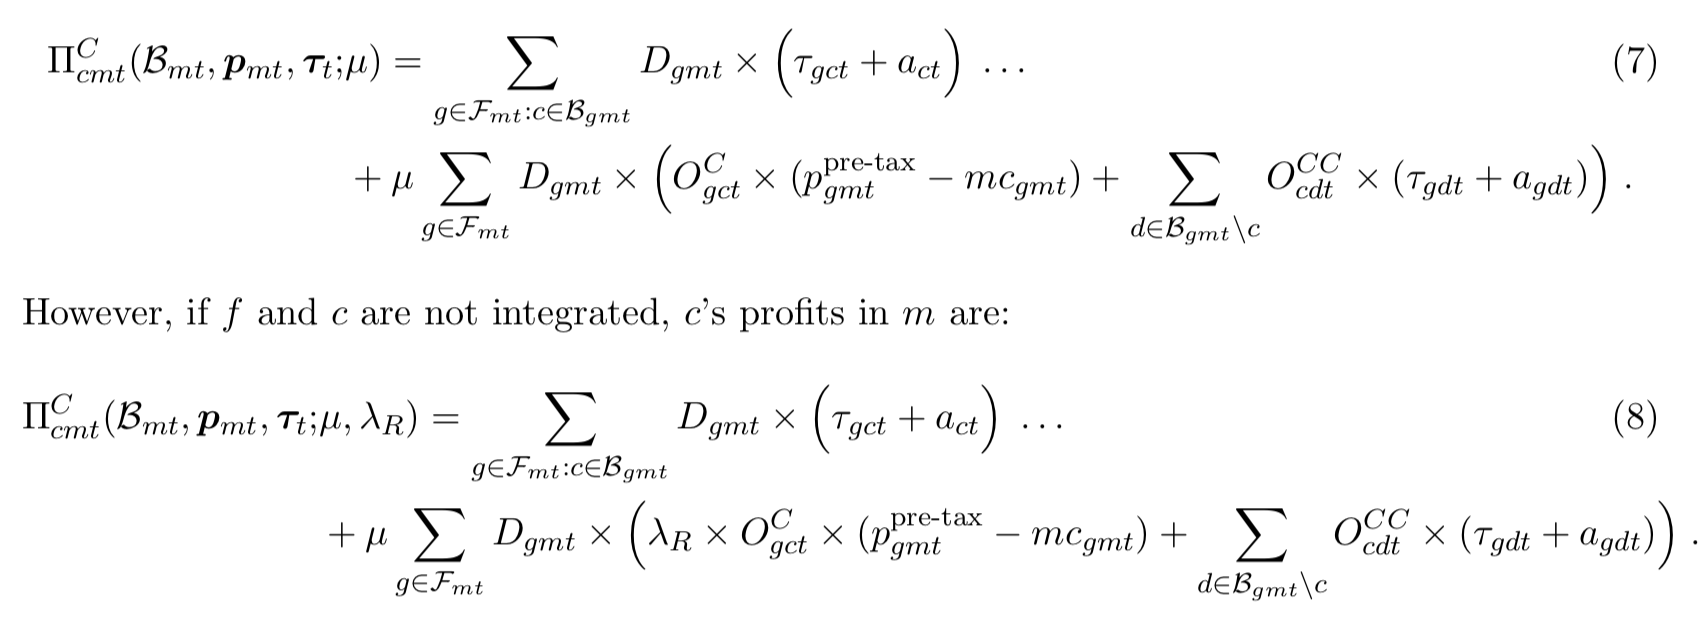
\includegraphics[width=4.5in]{./resources/mvpd1}
\end{center}
\begin{itemize}
\item Same as before $\mu$ is internalization of integrated profits
\item New parameter $\lambda_R$ is about \alert{raising rivals costs}.
\item Still get ad revenues but are different for channel and mvpd $a_{ct}$.
\end{itemize}

}

\frame[plain]{
\frametitle{Channel Payoffs / Bargaining}
\begin{center}
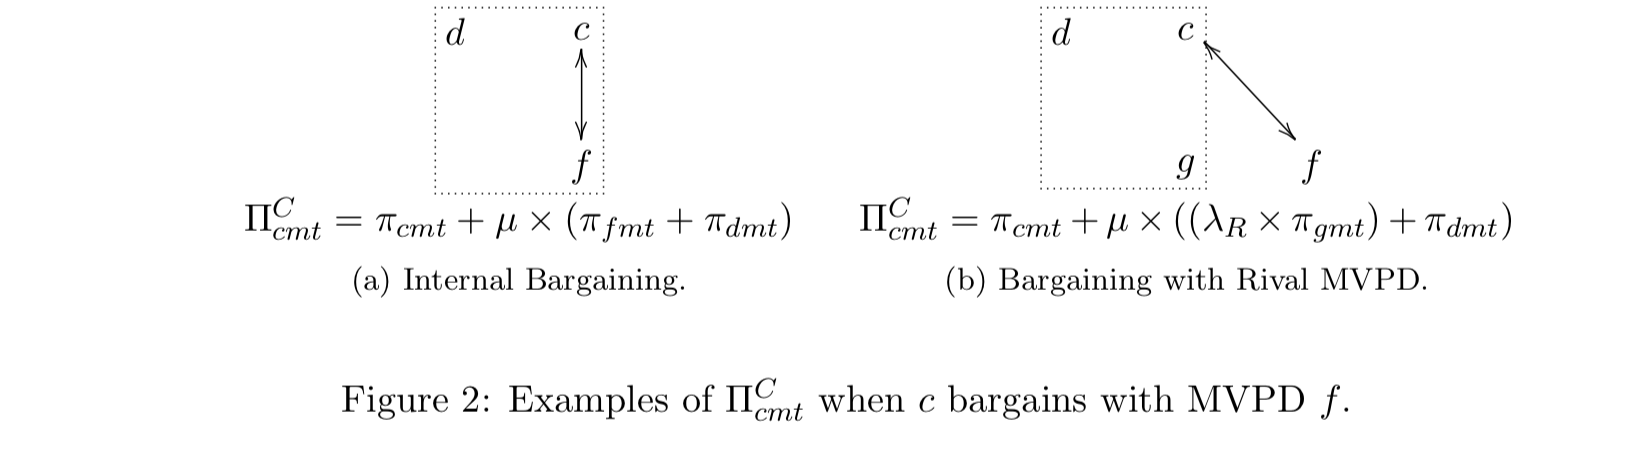
\includegraphics[width=5in]{./resources/mvpd2}
\end{center}
}


\frame[plain]{
\frametitle{Bargaining}
\begin{center}
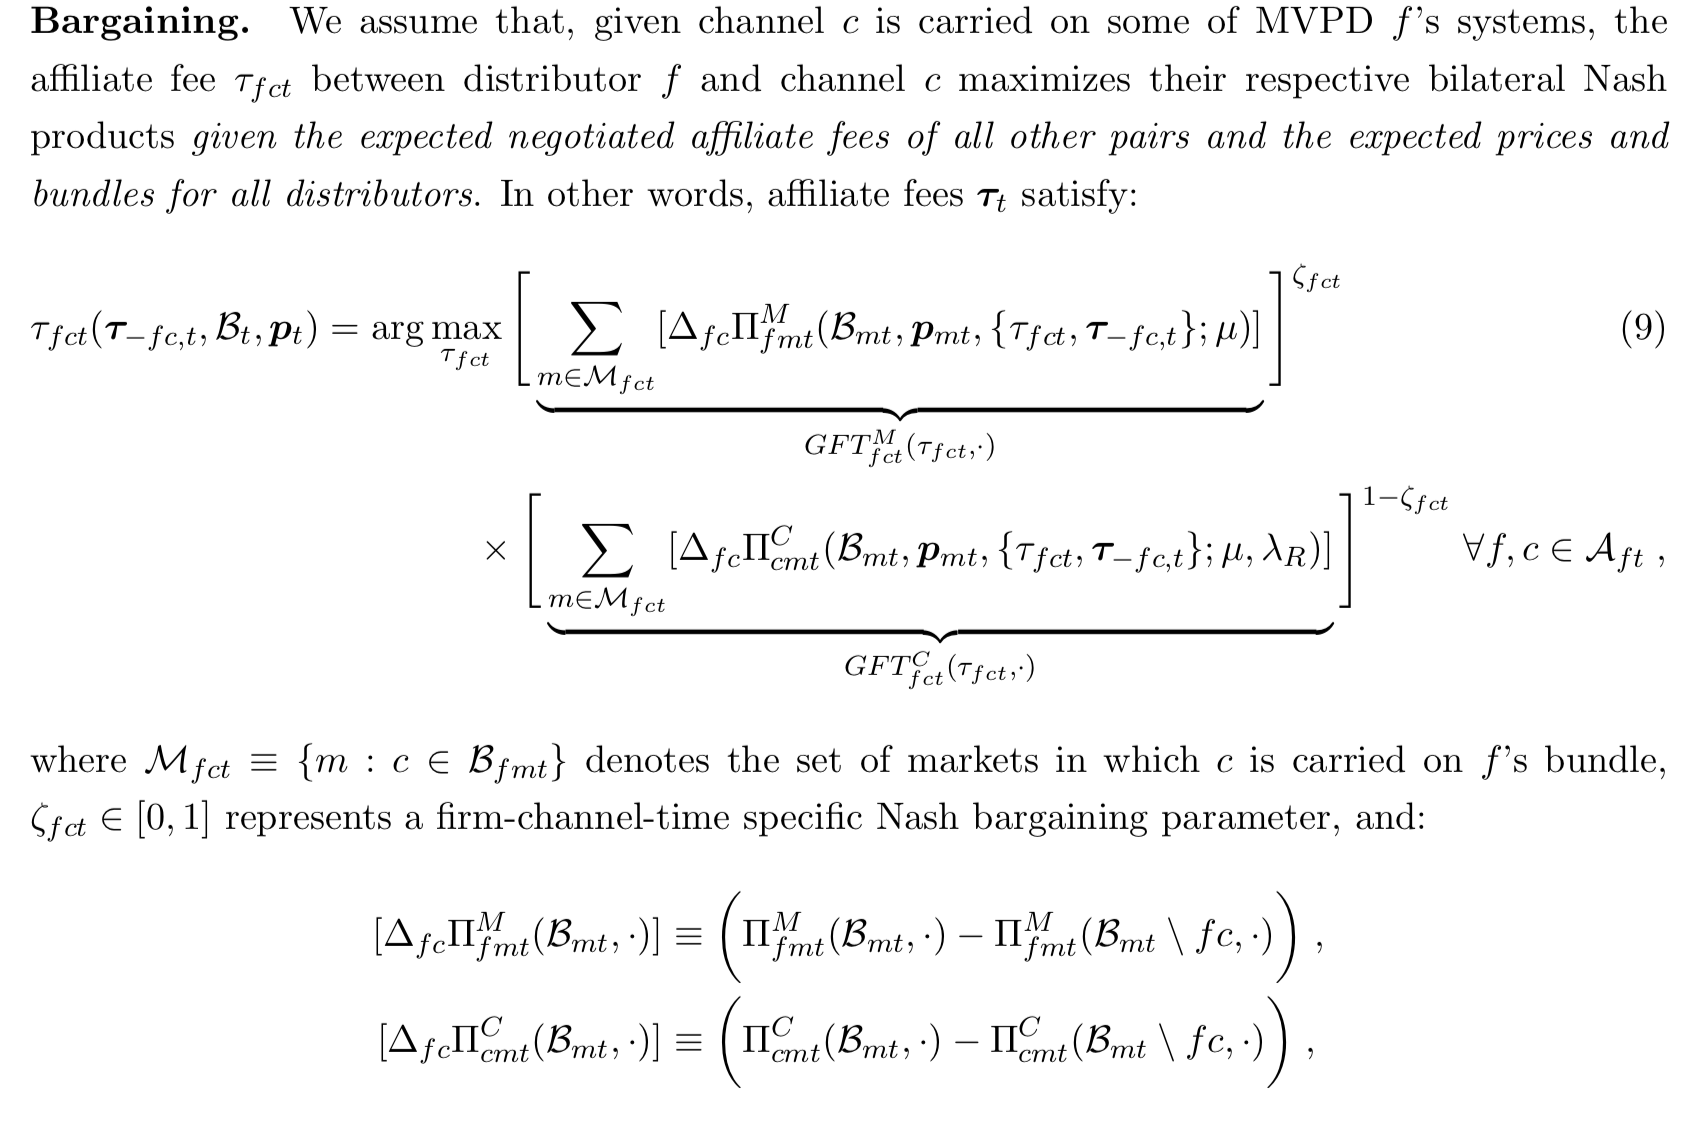
\includegraphics[width=4.5in]{./resources/mvpd3}
\end{center}
}

\frame[plain]{
\frametitle{Bargaining Example}
Ignore any vertical integration and think about just the bargaining:
\begin{center}
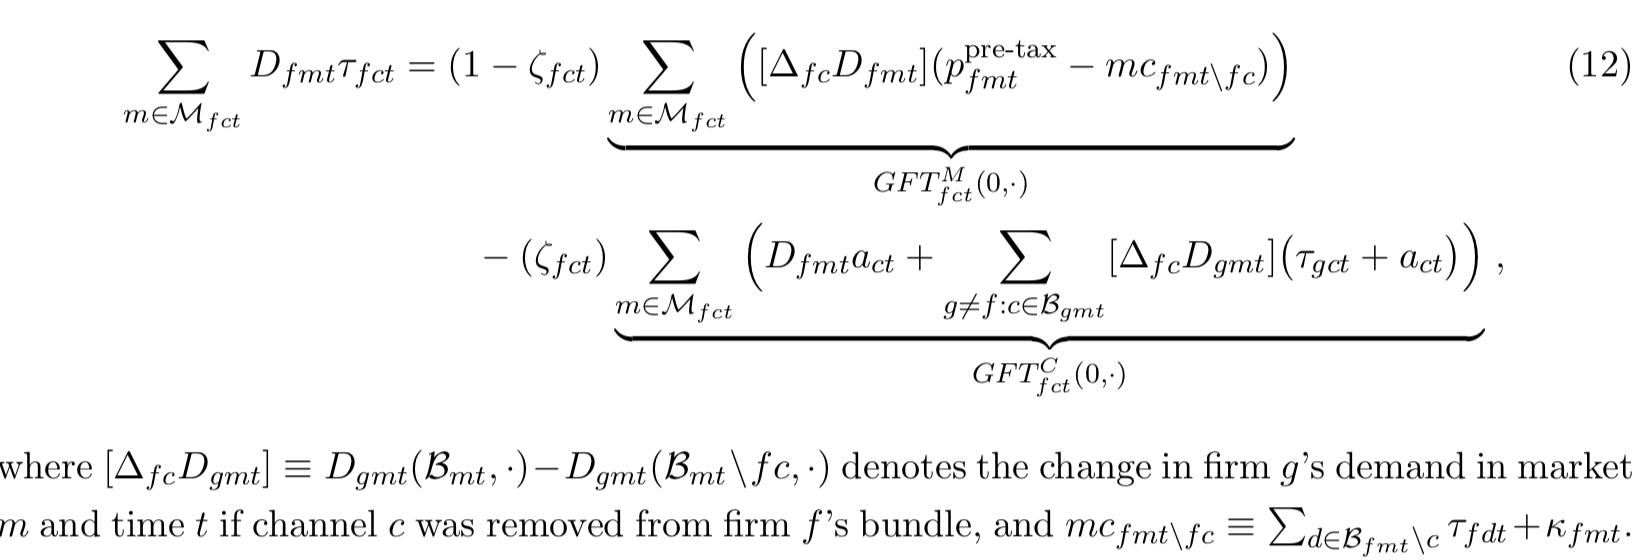
\includegraphics[width=4.5in]{./resources/mvpd4}
\begin{itemize}
\item Combined gains from trade from both $M$ and $C$
\item Last term is ``opportunity cost''.
\item Estimate two values for $\zeta \in \{\zeta^I, \zeta^E\}$.
\end{itemize}
\end{center}
}

\frame[plain]{
\frametitle{Nash in Nash Mechanics}
\begin{itemize}
\item Bargaining happens simultaneous with carriage and pricing
\item What this means is that if $\tau_{fct}$ changes then there is no change in $p_{fmt}$.
\begin{itemize}
\item Criticism is that this limits (but does not eliminate) mechanism for \alert{double marginalization} (by restricting what happens off the equilibrium path).
\item Sometimes criticized as ``schizophrenic'': division negotiating $\tau$ doesn't talk to local managers deciding $p_{fmt},\mathcal{B}_{fmt}$.
\end{itemize}
\item This is common in the literature: Grennan on Medical Devices, Ho or Ho and Lee on Hospitals-Insurers, Gowrisankaran, Nevo and Town on Hospitals-Insurers.
\item Collard-Wexler, Gowrisankaran and Lee (2017) attempt to micro-found the Nash-in-Nash solution.
\end{itemize}
}



\frame[plain]{
\frametitle{Double Marginalization}
Assume single channel $c$ fully owned by downstream firm $m$:
\begin{itemize}
\item Given $\tau$ firm $f$ sets the cable bundle price $p = \phi(mc_f + (1-\mu)\tau)$.
\begin{eqnarray*}
GFT_c^C(0,\cdot) &=&0  +  \mu \times (p - mc_f) D(p)\\
GFT_f^M(0,\cdot) &=& \mu \times (p - mc_f) D(p) + \mu \times 0
\end{eqnarray*}
\item The negotiated affiliate fee is then:
\begin{eqnarray*}
(1-\mu) \times D(p) = ( 1-\zeta)(p-mc_f) D(p) - \zeta \mu \times (p - mc_f) D(p)
\end{eqnarray*}
\item Holding $p$ fixed an increase in $\mu$ lowers $91-\mu)\tau$ (effective affiliate fee).
\item eq price satisfies $p = \phi(mc_f +[(1-\zeta) - \zeta \mu](p-mc_f))$.
\item Increasing $\mu$ lowers $p$.
\end{itemize}
}



\frame[plain]{
\frametitle{Identification}
\begin{center}
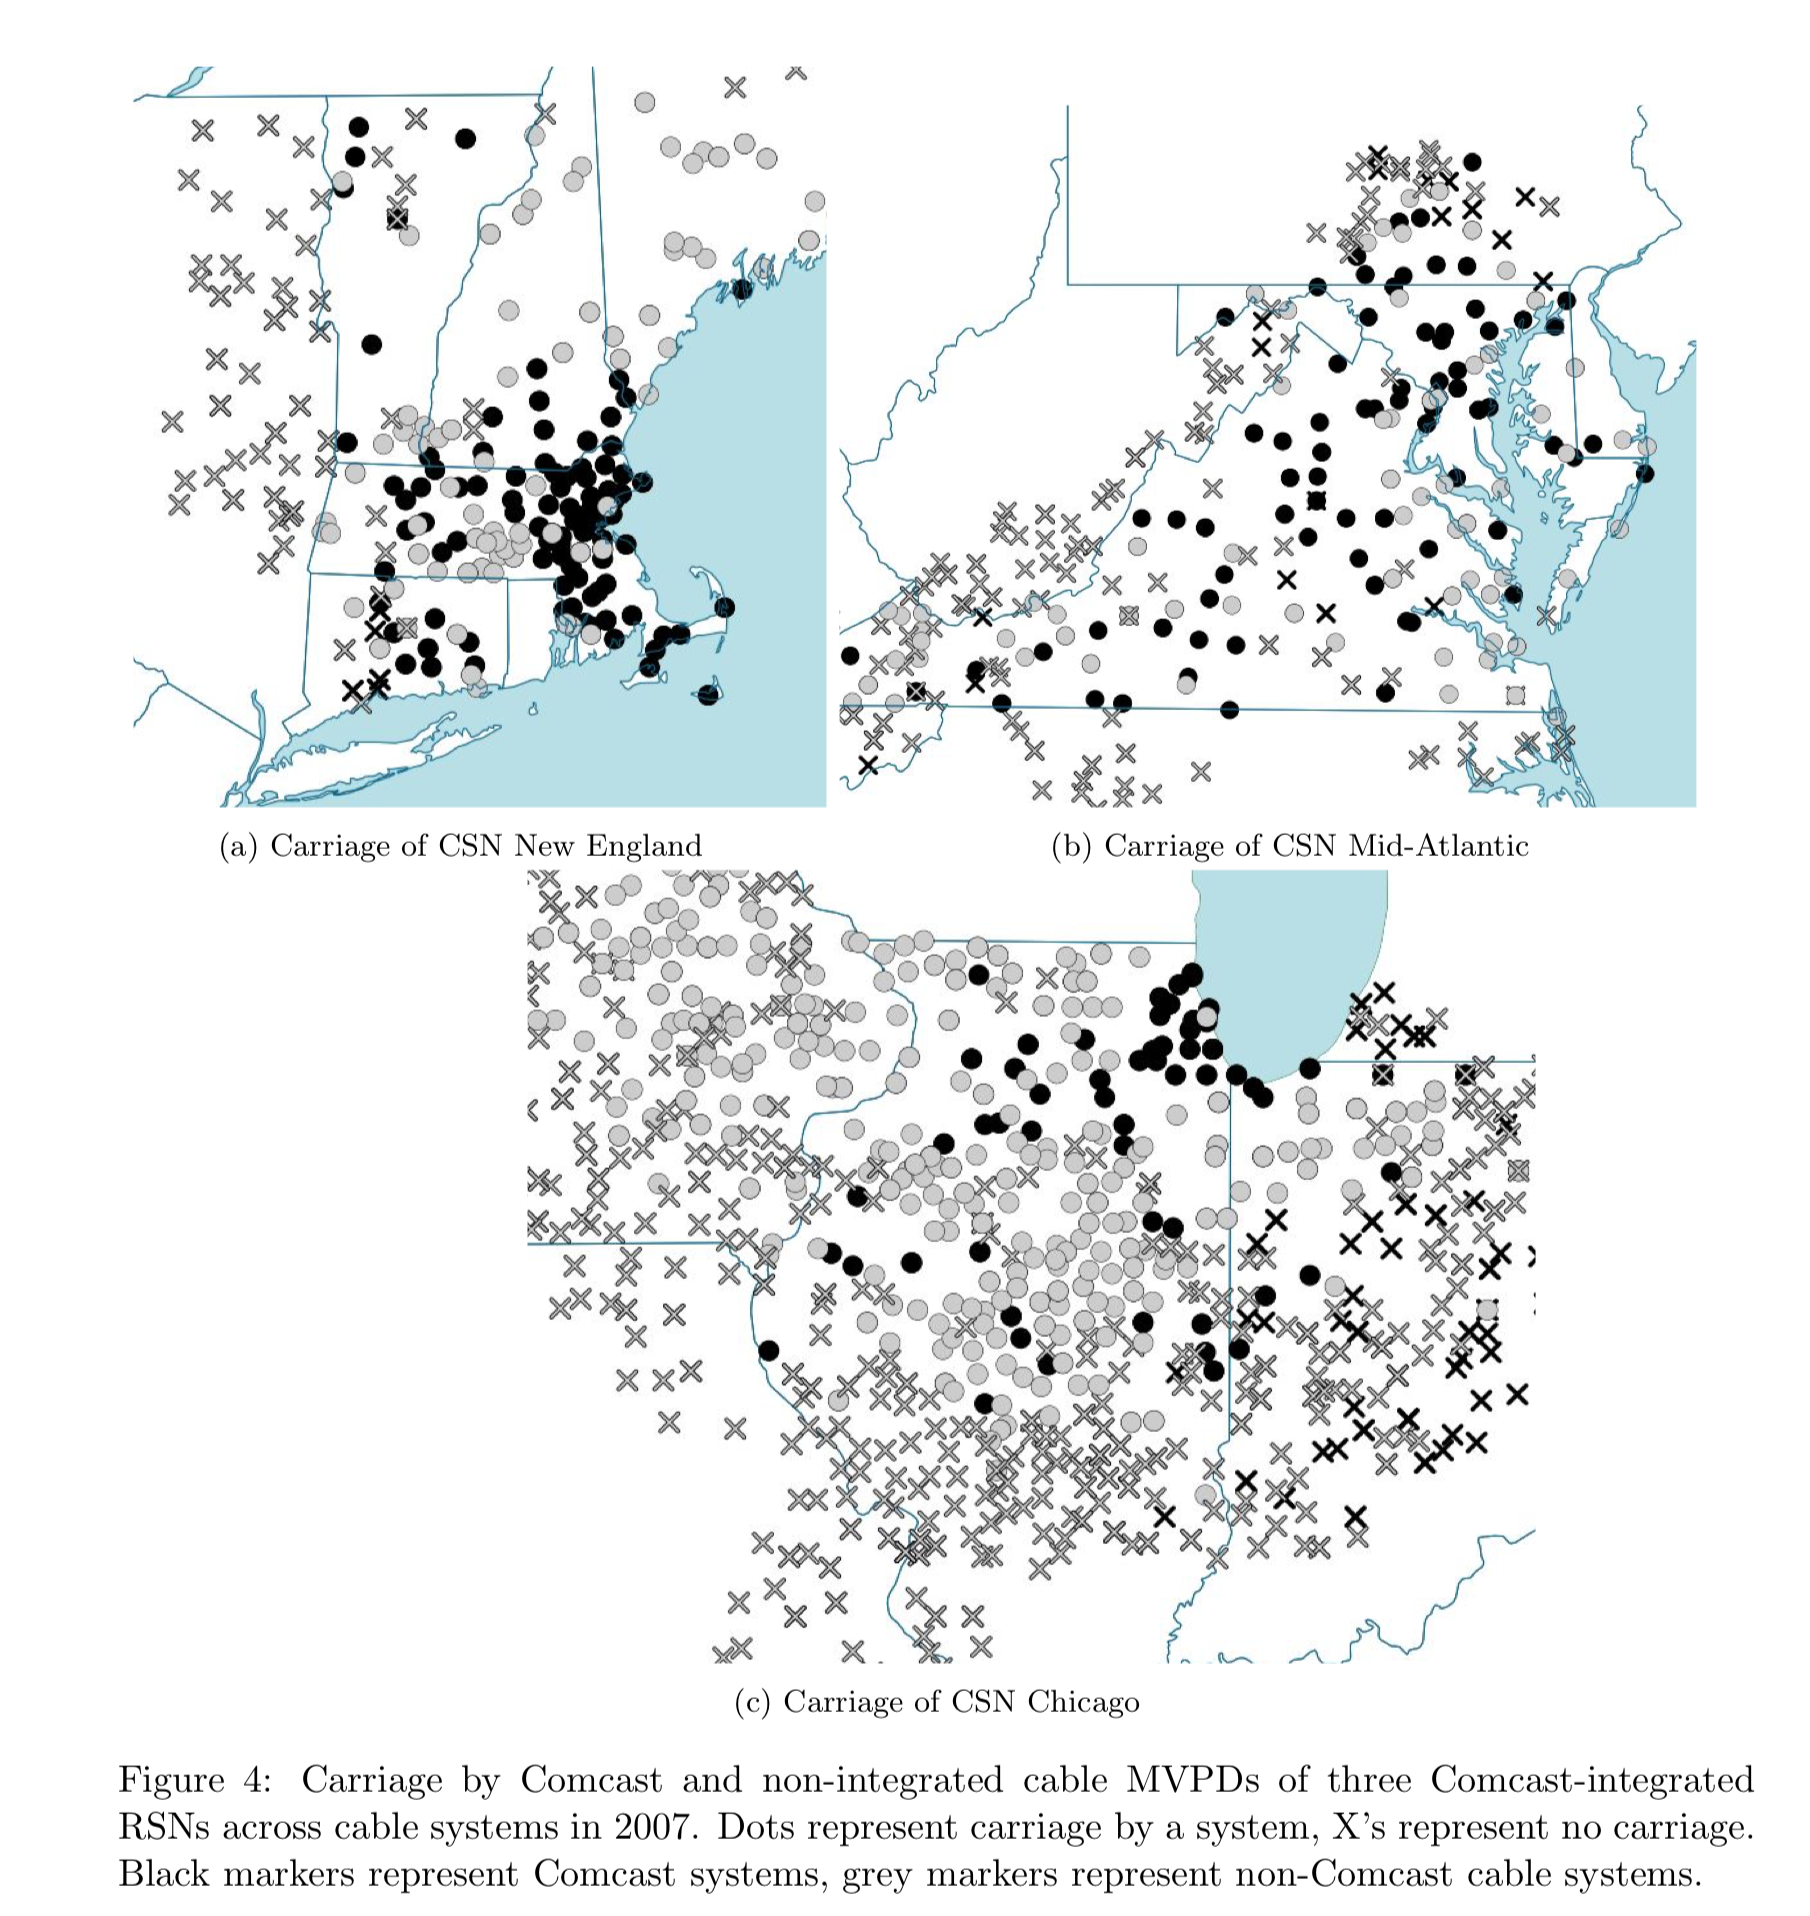
\includegraphics[width=3in]{./resources/mvpd5}
\end{center}
}

\frame[plain]{
\frametitle{  }
\begin{center}
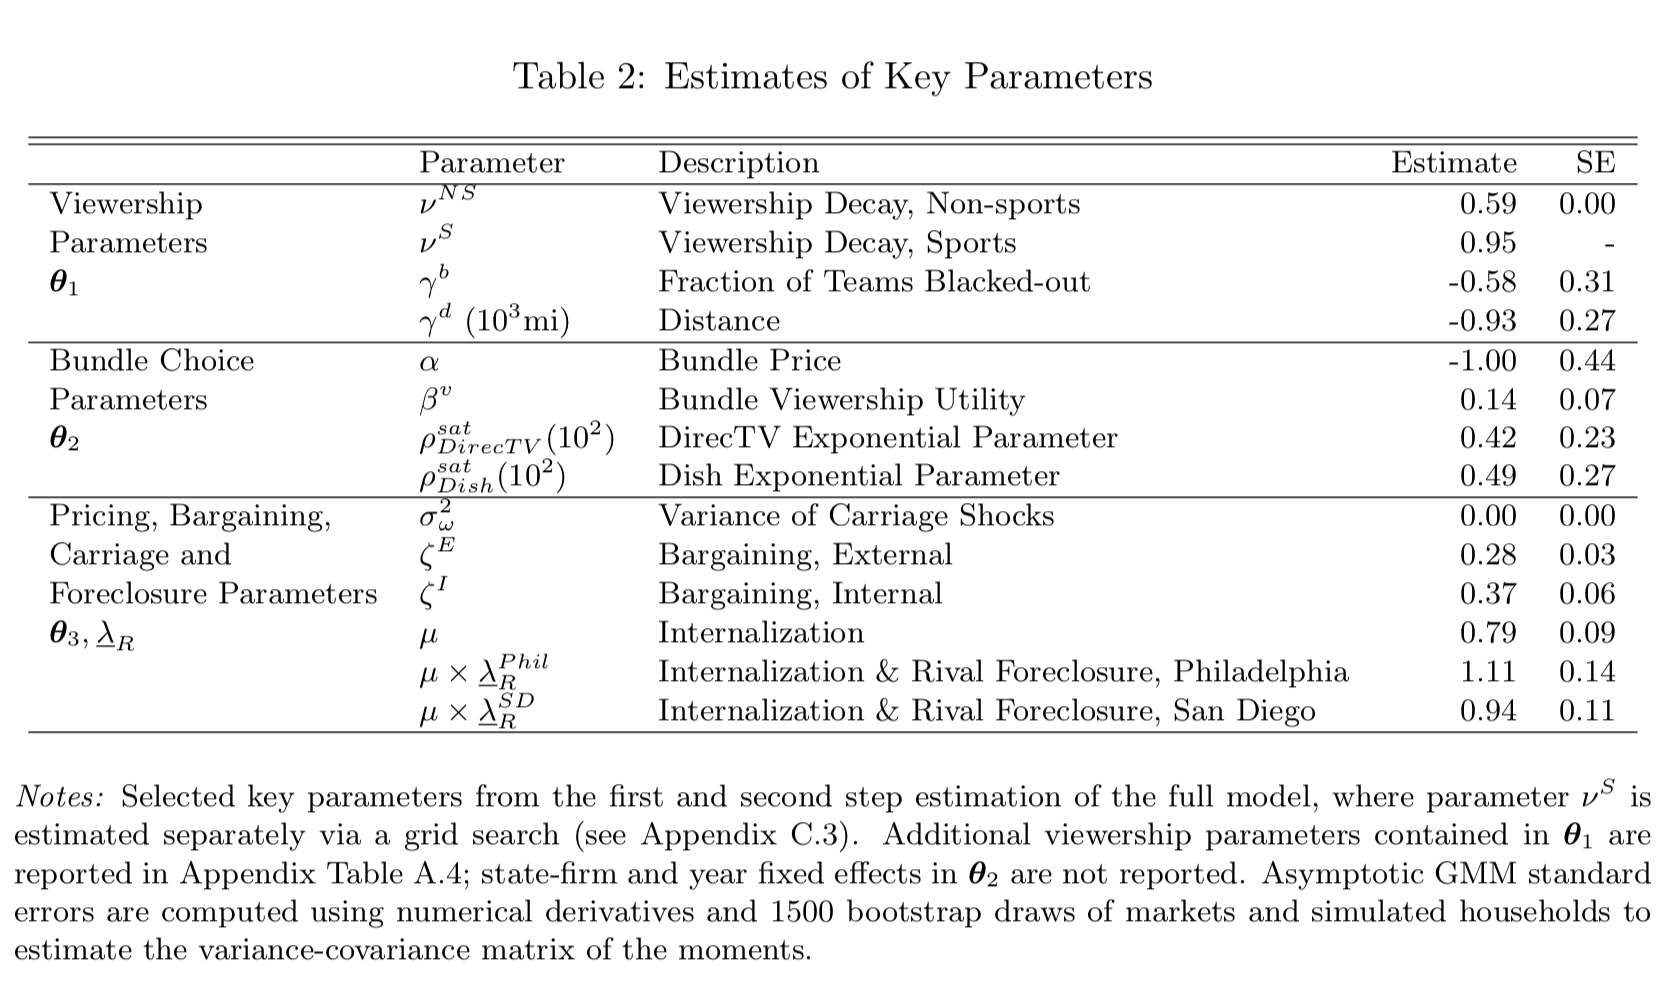
\includegraphics[width=4in]{./resources/mvpd6}
\end{center}
\begin{itemize}
\item Most markets have program access rules (PAR)s assume $\lambda_R = 0$.
\item Estimate lower bound on $\lambda_R$ because SAN and PHL have exclusion.
\end{itemize}
}

\frame[plain]{
\frametitle{ Results and Counterfactuals }
\begin{itemize}
\item Advantages of VI
\begin{itemize}
\item Lower negotiated price $\tau$ to cable company
\item Lower prices to consumers
\item More carriage by integrated firm
\end{itemize}
\item Disadvantages
\begin{itemize}
\item Higher prices to competitor (often satellite) $\tau$
\item Higher prices to competitor's customers $p$
\item Foreclosure or failure fo reach agreement.
\end{itemize}
\item Three scenarios
\begin{itemize}
\item No VI $(\mu=0)$.
\item VI with PARs $\lambda_R =0$
\item VI without PARs $\mu,\lambda_R$ both nonzero.
\end{itemize}
\end{itemize}
}

\frame[plain]{
\frametitle{Counterfactuals}
\begin{center}
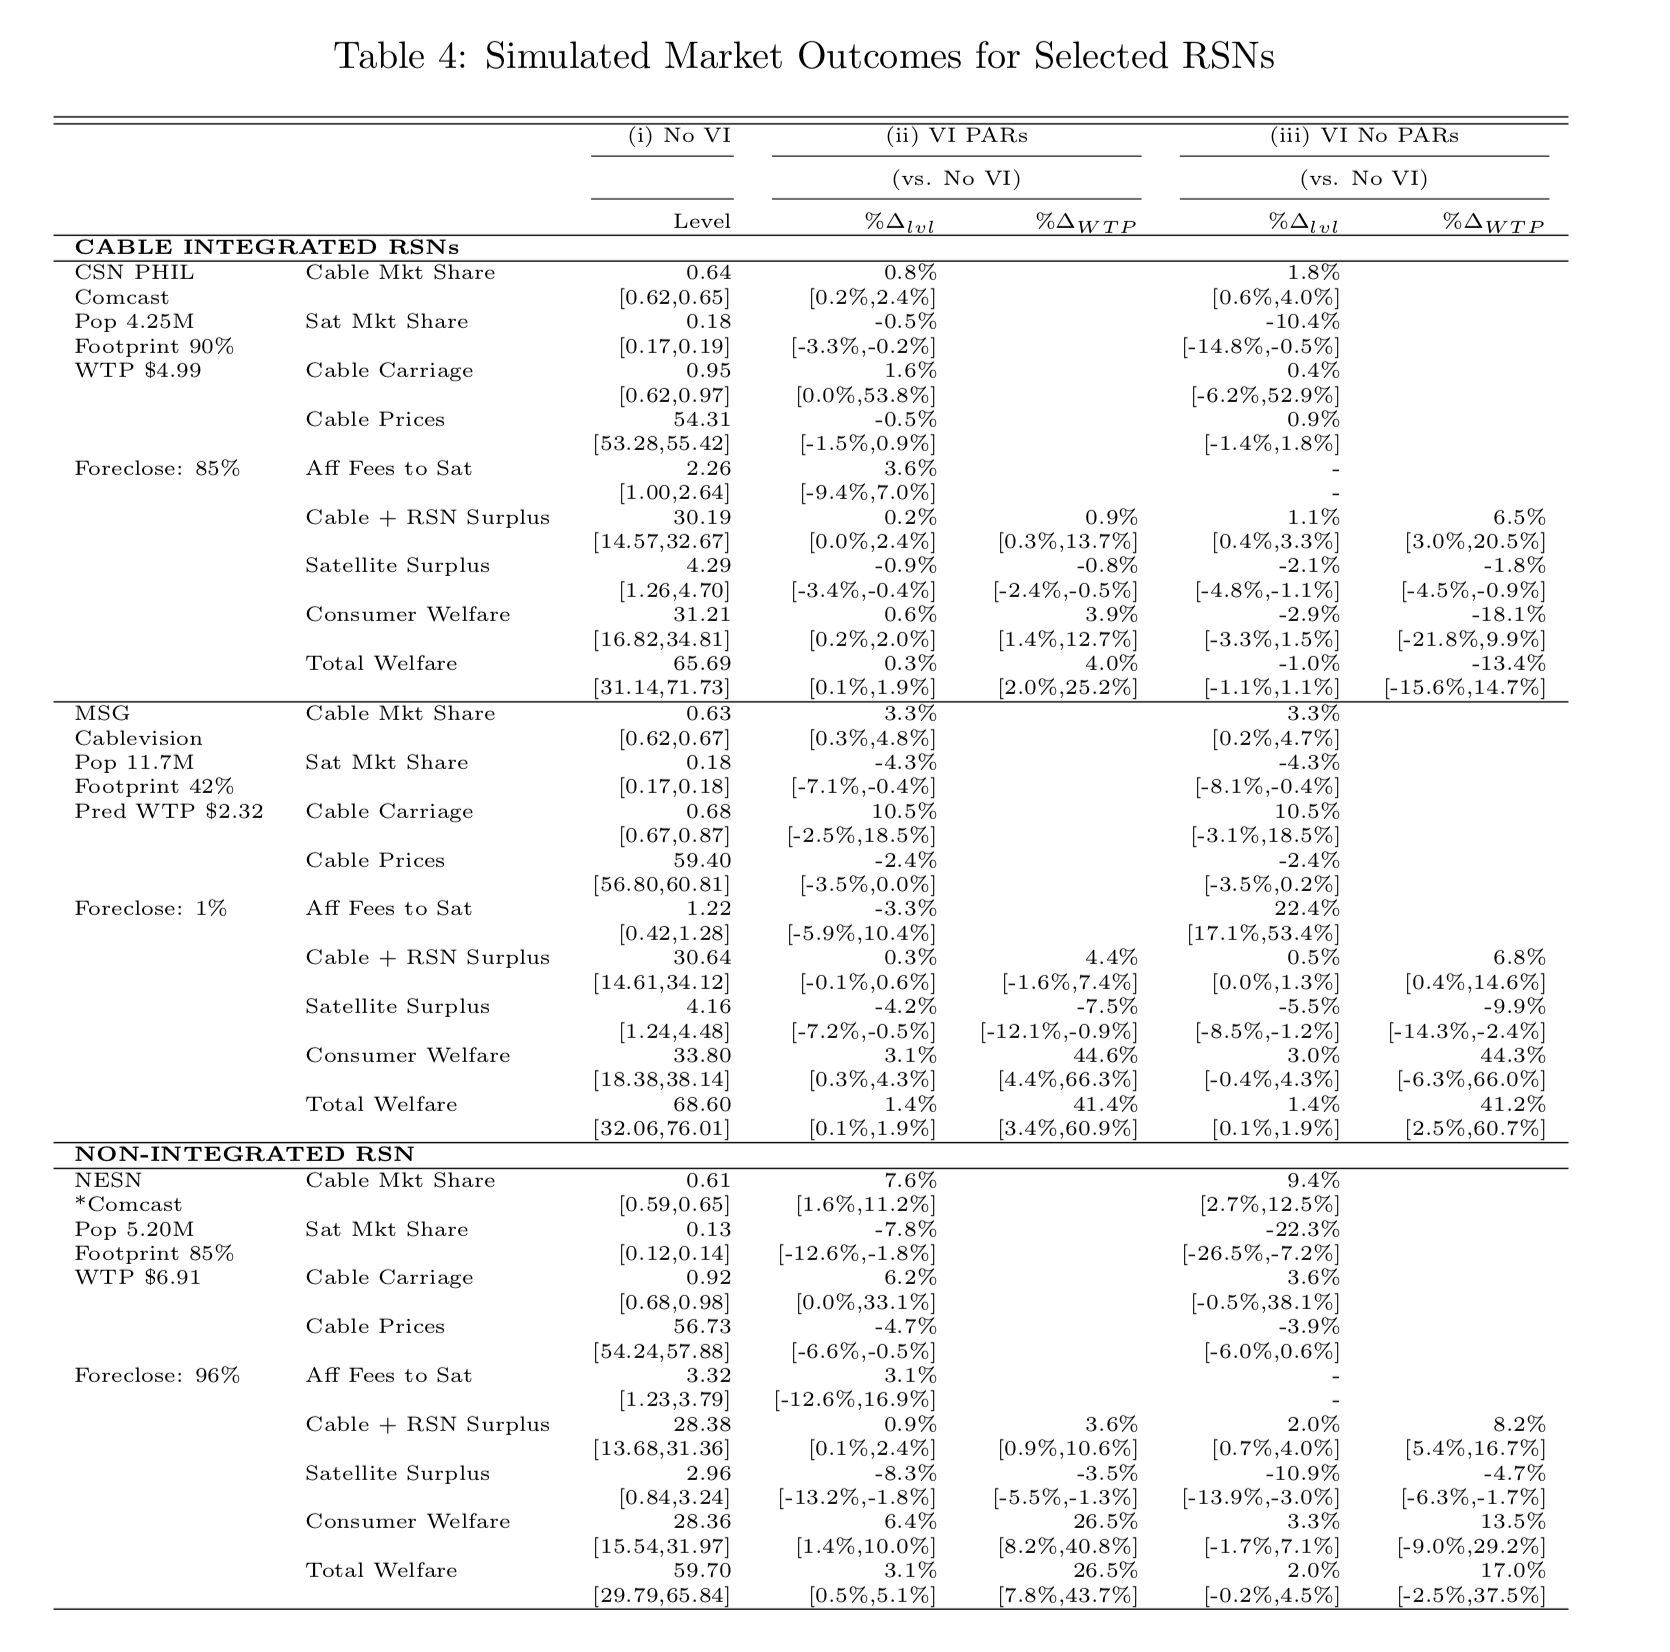
\includegraphics[width=3.25in]{./resources/mvpd7}
\end{center}
}



\frame[plain]{
\frametitle{ Conclusions }
\begin{itemize}
\item VI is good but PARs are important.
\end{itemize}
}

\end{document}